\chapter{Dynamic Programming}
\label{ch:dp}

Dynamic programming (DP) solves optimisation problems by combining solutions to overlapping subproblems. Unlike divide-and-conquer, which solves independent subproblems, DP reuses work---trading space for time and often reducing exponential search to polynomial time.

\section{The DP Paradigm}
\label{sec:dp-paradigm}

Two properties characterise problems amenable to DP.

\subsection{Optimal Substructure}

A problem has \emph{optimal substructure} if an optimal solution contains optimal solutions to its subproblems. Formally, let $S$ be an optimal solution to instance $I$ and let $I'$ be a sub-instance induced by $S$; then the restriction of $S$ to $I'$ is optimal for $I'$.

Not every optimisation problem qualifies. Longest \emph{simple} path in a general graph lacks optimal substructure---the subpath of a longest simple path need not be longest between its endpoints, because reusing vertices may be forbidden globally but not locally. DP is inapplicable there.

\subsection{Overlapping Subproblems}

A recursive formulation has \emph{overlapping subproblems} when the recursion tree revisits the same sub-instances many times. Naive recursion then does exponential work. DP stores each distinct subproblem result once.

\begin{table}[h]
\centering
\begin{tabular}{lll}
\toprule
Property & Divide \& Conquer & Dynamic Programming \\
\midrule
Subproblems & Independent / disjoint & Overlapping \\
Recomputation & None & Extensive without memo \\
Typical fix & -- & Memoisation or tabulation \\
\bottomrule
\end{tabular}
\caption{DP versus divide-and-conquer.}
\end{table}

\subsection{Memoisation versus Tabulation}

Both techniques achieve the same asymptotic bound; they differ in control flow.

\begin{itemize}
    \item \textbf{Memoisation (top-down):} Write the natural recursion and cache results in a dictionary or array on first computation. Only subproblems reachable from the initial call are solved. Recursion overhead and stack depth remain.
    \item \textbf{Tabulation (bottom-up):} Enumerate subproblems in order of increasing size and fill a table iteratively. No recursion; often better cache locality and easier complexity analysis.
\end{itemize}

\begin{lstlisting}[language=Python]
# memoised Fibonacci
memo = {0:0, 1:1}
def fib(n):
    if n not in memo:
        memo[n] = fib(n-1) + fib(n-2)
    return memo[n]

# tabulated Fibonacci
def fib_tab(n):
    dp = [0]*(n+1); dp[1]=1
    for i in range(2, n+1):
        dp[i] = dp[i-1] + dp[i-2]
    return dp[n]
\end{lstlisting}

Tabulation is preferred in this course because it makes the dependency structure explicit, which we exploit to reconstruct solutions.

%------------------------------------------------------------------
\section{Longest Common Subsequence}
\label{sec:lcs}

Given $X = x_1\ldots x_m$ and $Y = y_1\ldots y_n$, a \emph{subsequence} deletes zero or more characters. The LCS problem asks for a longest sequence that is a subsequence of both $X$ and $Y$.

\subsection{Optimal Substructure and Recurrence}

Let $c[i][j]$ be the LCS length of $X_i = x_1\ldots x_i$ and $Y_j = y_1\ldots y_j$, with $c[0][j]=c[i][0]=0$.

\[
c[i][j] =
\begin{cases}
c[i-1][j-1]+1 & \text{if } x_i = y_j,\\[4pt]
\max\{c[i-1][j],\, c[i][j-1]\} & \text{if } x_i \neq y_j.
\end{cases}
\]

If $x_i = y_j$, any LCS must end with that character and extend an LCS of $X_{i-1},Y_{j-1}$. If $x_i\neq y_j$, an LCS discards either $x_i$ or $y_j$. Overlapping subproblems are immediate: $c[i][j]$ depends on three neighbours, so naive recursion re-evaluates the same cells exponentially many times.

\subsection{Tabulation and Walkthrough}

Filling row by row gives $O(mn)$ time and $O(mn)$ space. We also store a direction $b[i][j]\in\{\diagup,\uparrow,\leftarrow\}$ to reconstruct an LCS by backtracking from $c[m][n]$.

Take $X=\langle A,B,C\rangle$, $Y=\langle A,C,B\rangle$ ($m=n=3$):

\begin{center}
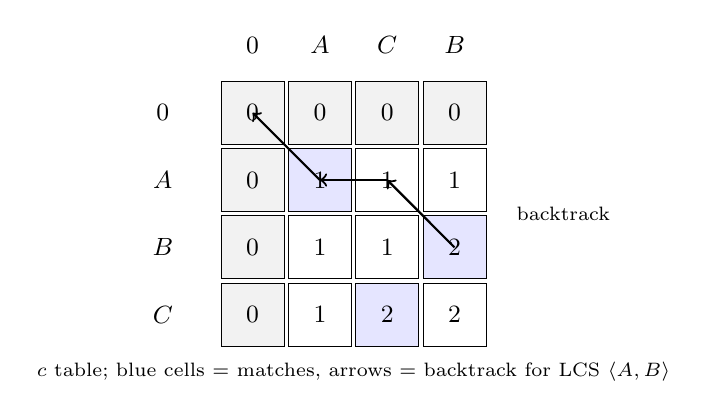
\begin{tikzpicture}[scale=0.95, every node/.style={font=\small}]
\tikzset{cell/.style={minimum size=8mm, draw, anchor=center}}
% grid labels
\node at (-1.2,0) {$0$}; \node at (-1.2,-0.9) {$A$}; \node at (-1.2,-1.8) {$B$}; \node at (-1.2,-2.7) {$C$};
\node at (0,0.9) {$0$}; \node at (0.9,0.9) {$A$}; \node at (1.8,0.9) {$C$}; \node at (2.7,0.9) {$B$};
% row 0
\node[cell,fill=gray!10] at (0,0) {0}; \node[cell,fill=gray!10] at (0.9,0) {0}; \node[cell,fill=gray!10] at (1.8,0) {0}; \node[cell,fill=gray!10] at (2.7,0) {0};
% row A
\node[cell,fill=gray!10] at (0,-0.9) {0}; \node[cell,fill=blue!10] at (0.9,-0.9) {1}; \node[cell] at (1.8,-0.9) {1}; \node[cell] at (2.7,-0.9) {1};
% row B
\node[cell,fill=gray!10] at (0,-1.8) {0}; \node[cell] at (0.9,-1.8) {1}; \node[cell] at (1.8,-1.8) {1}; \node[cell,fill=blue!10] at (2.7,-1.8) {2};
% row C
\node[cell,fill=gray!10] at (0,-2.7) {0}; \node[cell] at (0.9,-2.7) {1}; \node[cell,fill=blue!10] at (1.8,-2.7) {2}; \node[cell] at (2.7,-2.7) {2};
% arrows for one LCS path A->B
\draw[->,thick] (2.7,-1.8) -- (1.8,-0.9);
\draw[->,thick] (1.8,-0.9) -- (0.9,-0.9);
\draw[->,thick] (0.9,-0.9) -- (0,0);
\node[font=\scriptsize, right] at (3.4,-1.35) {backtrack};
\node[font=\scriptsize, below] at (1.35,-3.2) {$c$ table; blue cells = matches, arrows = backtrack for LCS $\langle A,B\rangle$};
\end{tikzpicture}
\end{center}

Filling order: $c[1][1]=1$ ($A{=}A$, diagonal $+1$), $c[1][2]=1$ ($\max(0,1)$), $c[1][3]=1$, $c[2][3]=2$ ($B{=}B$). Backtracking from $c[3][3]=2$ follows the arrows above to recover $\langle A,B\rangle$ (equivalently $\langle A,C\rangle$ via a different tie-break).

Reconstruction is $O(m+n)$: start at $(m,n)$; on $\diagup$ output $x_i$ and move to $(i-1,j-1)$; on $\uparrow$ move to $(i-1,j)$; on $\leftarrow$ move to $(i,j-1)$.

%------------------------------------------------------------------
\section{0/1 Knapsack}
\label{sec:knapsack}

Given $n$ items with weights $w_i$, values $v_i$, and capacity $W$, choose a subset maximising total value without exceeding $W$. Each item is taken at most once.

Let $K[i][w]$ be the optimum value using items $1\ldots i$ with capacity $w$, where $K[0][w]=K[i][0]=0$:

\[
K[i][w] =
\begin{cases}
K[i-1][w] & \text{if } w_i > w,\\
\max\{K[i-1][w],\; K[i-1][w-w_i]+v_i\} & \text{otherwise.}
\end{cases}
\]

Either item $i$ is excluded (value $K[i-1][w]$) or included (value $K[i-1][w-w_i]+v_i$). Time $O(nW)$, space $O(nW)$---pseudo-polynomial in $W$.

\subsection{Table and Backtracking}

Example: $W=5$, items $(w,v)$: $1:(2,3), 2:(3,4), 3:(4,5), 4:(5,6)$.

\begin{center}
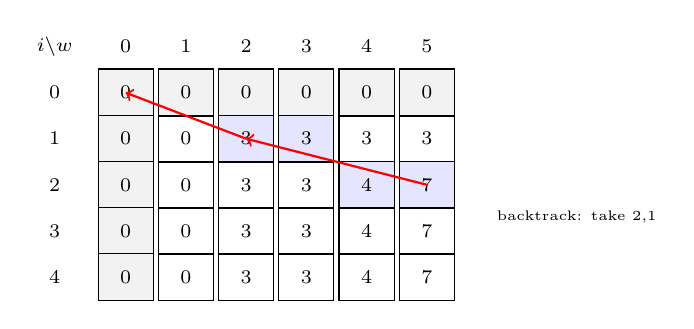
\begin{tikzpicture}[scale=0.9, every node/.style={font=\scriptsize}]
\tikzset{cell/.style={minimum width=7mm, minimum height=6mm, draw, anchor=center}}
% header
\node at (-1.0,0) {$i\backslash w$}; \foreach \w in {0,...,5} \node at (\w*0.85,0) {\w};
% row 0
\node at (-1.0,-0.65) {0}; \foreach \w in {0,...,5} \node[cell,fill=gray!10] at (\w*0.85,-0.65) {0};
% row 1
\node at (-1.0,-1.3) {1}; \node[cell,fill=gray!10] at (0,-1.3) {0}; \node[cell] at (0.85,-1.3) {0}; \node[cell,fill=blue!10] at (1.7,-1.3) {3}; \node[cell,fill=blue!10] at (2.55,-1.3) {3}; \node[cell] at (3.4,-1.3) {3}; \node[cell] at (4.25,-1.3) {3};
% row 2
\node at (-1.0,-1.95) {2}; \node[cell,fill=gray!10] at (0,-1.95) {0}; \node[cell] at (0.85,-1.95) {0}; \node[cell] at (1.7,-1.95) {3}; \node[cell] at (2.55,-1.95) {3}; \node[cell,fill=blue!10] at (3.4,-1.95) {4}; \node[cell,fill=blue!10] at (4.25,-1.95) {7};
% row 3
\node at (-1.0,-2.6) {3}; \node[cell,fill=gray!10] at (0,-2.6) {0}; \node[cell] at (0.85,-2.6) {0}; \node[cell] at (1.7,-2.6) {3}; \node[cell] at (2.55,-2.6) {3}; \node[cell] at (3.4,-2.6) {4}; \node[cell] at (4.25,-2.6) {7};
% row 4
\node at (-1.0,-3.25) {4}; \node[cell,fill=gray!10] at (0,-3.25) {0}; \node[cell] at (0.85,-3.25) {0}; \node[cell] at (1.7,-3.25) {3}; \node[cell] at (2.55,-3.25) {3}; \node[cell] at (3.4,-3.25) {4}; \node[cell] at (4.25,-3.25) {7};
\draw[->,thick,red] (4.25,-1.95) -- (1.7,-1.3); \draw[->,thick,red] (1.7,-1.3) -- (0,-0.65);
\node[font=\tiny, right] at (5.1,-2.4) {backtrack: take 2,1};
\end{tikzpicture}
\end{center}

Optimum $K[4][5]=7$ (items $1{+}2$, weight $5$). Backtrack: if $K[i][w]\neq K[i-1][w]$, item $i$ was taken; move to $w-w_i$, else move to $i-1$. Space can be reduced to $O(W)$ with a 1-D array iterated backwards, but backtracking then needs the full table or stored decisions.

%------------------------------------------------------------------
\section{Matrix Chain Multiplication}
\label{sec:matrix-chain}

Given matrices $A_1\ldots A_n$ where $A_i$ is $p_{i-1}\times p_i$, the cost of multiplying $A_i\cdots A_j$ depends on parenthesisation. Multiplying $p\times q$ by $q\times r$ costs $pqr$ scalar multiplications.

Let $m[i][j]$ be the minimum cost to compute $A_i\cdots A_j$, with $m[i][i]=0$:

\[
m[i][j] = \min_{i\le k < j} \bigl\{m[i][k] + m[k+1][j] + p_{i-1}\,p_k\,p_j\bigr\}.
\]

We also store $s[i][j]=k$ achieving the minimum to reconstruct the parenthesisation. There are $\Theta(n^2)$ subproblems, each trying $O(n)$ splits: $O(n^3)$ time, $O(n^2)$ space. Fill by increasing chain length $l=2\ldots n$.

Example: $p=(10,30,5,60)$ for $A_1(10{\times}30),A_2(30{\times}5),A_3(5{\times}60)$. Then $m[2][3]=30{\cdot}5{\cdot}60=9000$, $m[1][2]=10{\cdot}30{\cdot}5=1500$, and $m[1][3]=\min\{m[1][1]+m[2][3]+10{\cdot}30{\cdot}60=0+9000+18000,\,m[1][2]+m[3][3]+10{\cdot}5{\cdot}60=1500+0+3000\}=4500$ with $k=2$, i.e.\\ $(A_1A_2)A_3$.

\begin{center}
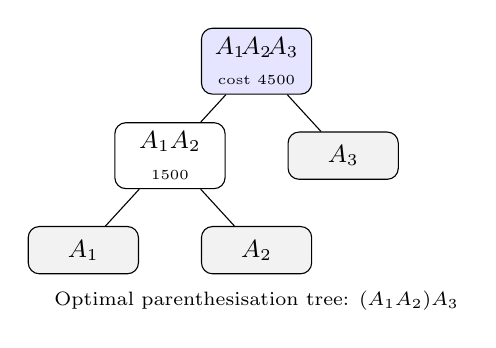
\begin{tikzpicture}[every node/.style={font=\small}, level distance=12mm, sibling distance=22mm,
  box/.style={draw, rounded corners, minimum width=14mm, minimum height=6mm, align=center}]
\node[box,fill=blue!10] {$A_1\!A_2\!A_3$ \\ \tiny cost $4500$}
  child {node[box] {$A_1A_2$ \\ \tiny $1500$}
    child {node[box,fill=gray!10] {$A_1$}}
    child {node[box,fill=gray!10] {$A_2$}}
  }
  child {node[box,fill=gray!10] {$A_3$}};
\node[font=\scriptsize, below] at (0,-2.8) {Optimal parenthesisation tree: $(A_1A_2)A_3$};
\end{tikzpicture}
\end{center}

%------------------------------------------------------------------
\section{Coin Change: Unbounded Knapsack}
\label{sec:coin-change-dp}

Given coin denominations $d_1\ldots d_k$ (unlimited supply) and amount $N$, find the minimum number of coins to make $N$ (or report impossible).

Let $\mathit{dp}[x]$ be the minimum coins for amount $x$, with $\mathit{dp}[0]=0$ and $\mathit{dp}[x]=\infty$ for $x<0$ initially. For $x\ge 1$:

\[
\mathit{dp}[x] = 1 + \min_{d_i\le x} \mathit{dp}[x-d_i],
\]
taking $\infty$ if no $d_i\le x$ yields a finite predecessor. Equivalently, tabulate $x=1\ldots N$ and for each coin $d_i$ relax $\mathit{dp}[x]$ from $\mathit{dp}[x-d_i]$.

This is unbounded knapsack: each coin may be reused, so the recurrence looks back at the same coin set (contrast 0/1 knapsack which moves to $i-1$). Time $O(kN)$, space $O(N)$. Reconstruct coins by storing $\mathit{choice}[x]$, the first coin used.

Example: $d=(1,3,4)$, $N=6$. Then $\mathit{dp}$ is $0,1,2,1,1,2,2$ for $x=0\ldots 6$; e.g.\ $\mathit{dp}[6]=1+\min(\mathit{dp}[5],\mathit{dp}[3],\mathit{dp}[2])=1+1=2$ via $3+3$. Greedy (always take largest $d_i\le x$) fails here: it gives $4+1+1$ (3 coins).

\begin{lstlisting}[language=Python]
def coin_change(coins, N):
    INF = N+1
    dp = [INF]*(N+1); choice=[-1]*(N+1)
    dp[0]=0
    for x in range(1, N+1):
        for c in coins:
            if c<=x and dp[x-c]+1 < dp[x]:
                dp[x]=dp[x-c]+1; choice[x]=c
    return dp[N] if dp[N]!=INF else -1  # -1 = impossible
\end{lstlisting}

The same table answers counting variants: number of ways uses $\mathit{ways}[x]+= \mathit{ways}[x-d_i]$ with careful ordering to avoid permuting combinations.

%------------------------------------------------------------------
\section{Exercises}
\label{sec:dp-exercises}

\begin{enumerate}
    \item \textbf{LCS by hand.} Compute the full $c$ and $b$ tables for $X=\langle B,D,C,A\rangle$, $Y=\langle A,B,C,D\rangle$. List all distinct LCSs and trace each backtracking path.

    \item \textbf{Knapsack trace.} For capacity $W=6$ and items $(w,v)=(1,1),(2,4),(3,4),(4,5)$, fill the $K$ table, state the optimum value, and backtrack to find every optimal subset. Then give the $O(W)$-space tabulated code and explain why the inner loop must run backwards.

    \item \textbf{Matrix chain.} Let $p=(5,10,3,12,5)$. Compute all $m[i][j]$ and $s[i][j]$ by hand, give the optimal parenthesisation and its cost, and argue why the greedy choice of cheapest single multiplication first is not optimal.

    \item \textbf{Coin change variants.} With $d=(1,3,4)$ and $N=6$, (a) show the $\mathit{dp}$ table and the coins chosen, (b) give a counterexample where greedy fails for $d=(1,7,10)$, and (c) modify the DP to count the number of distinct combinations (order irrelevant) and compute it for $N=6$.

    \item \textbf{Edit distance (DP design).} Define edit distance with operations insert, delete, replace (cost $1$). Derive the recurrence for $\mathit{ed}[i][j]$ on prefixes, state the table size and filling order, and adapt the algorithm to output an optimal edit sequence.
\end{enumerate}
